% Created 2017-03-09 Thu 16:18
% Intended LaTeX compiler: pdflatex
\documentclass[a4paper,11pt]{article}
\usepackage[utf8]{inputenc}
\usepackage[T1]{fontenc}
\usepackage{graphicx}
\usepackage{grffile}
\usepackage{longtable}
\usepackage{wrapfig}
\usepackage{rotating}
\usepackage[normalem]{ulem}
\usepackage{amsmath}
\usepackage{textcomp}
\usepackage{amssymb}
\usepackage{capt-of}
\usepackage{hyperref}
\renewcommand\maketitle{
  \begin{titlepage}
    \centering
    \vfill
    
\includegraphics{images/pexip_logo.png}
    \vspace*{\stretch{1.0}}
    \begin{center}
      \large\textbf{Building Native WebRTC Applications against the Pexip client API}\\
      \large\textit{Ian Mortimer}
      \large\textit{- ian@pexip.com}
    \end{center}
    \vspace*{\stretch{2.0}}
    \vfill
  \end{titlepage}
}

\usepackage[margin=1in]{geometry}
\usepackage[hyperref,x11names]{xcolor}
\usepackage[colorlinks=true,urlcolor=SteelBlue4,linkcolor=Firebrick4]{hyperref}
\usepackage[T1]{fontenc}
\usepackage[scaled]{beraserif}
\usepackage[scaled]{berasans}
\usepackage[scaled]{beramono}
\usepackage{microtype}
\usepackage{amssymb,amsmath}
\usepackage{fancyhdr} %For headers and footers
\pagestyle{fancy} %For headers and footers
\usepackage{lastpage} %For getting page x of y
\usepackage{float} %Allows the figures to be positioned and formatted nicely
\restylefloat{figure} %and this command
\usepackage{url} %Formatting of yrls
\lhead{}
\chead{}
\rhead{Building Native WebRTC Apps}
\lfoot{Pexip AS | Registered Company Number: BR015978}
\cfoot{}
\rfoot{Page \thepage}
\usepackage{xcolor}
\PassOptionsToPackage{hyperref,x11names}{xcolor}
\definecolor{electricblue}{HTML}{0D2E63}
\usepackage{tocloft}
\usepackage{microtype}
\renewcommand{\cftsecleader}{\cftdotfill{\cftdotsep}}
\usepackage[breaklinks=true,linktocpage,xetex]{hyperref}
\hypersetup{colorlinks, citecolor=electricblue,filecolor=electricblue,linkcolor=electricblue,urlcolor=electricblue}
\author{Ian Mortimer}
\date{\today}
\title{Building native WebRTC applicationsls against Pexip client API}
\hypersetup{
 pdfauthor={Ian Mortimer},
 pdftitle={Building native WebRTC applicationsls against Pexip client API},
 pdfkeywords={},
 pdfsubject={},
 pdfcreator={Emacs 25.1.1 (Org mode 9.0.4)}, 
 pdflang={English}}
\begin{document}

\maketitle
\tableofcontents

\clearpage

\section{Introduction}
\label{sec:orgc51bdba}

In the following article, we'll be covering the steps required to
build a complete working WebRTC based video and chat application using
the Pexip client REST API and native builds of WebRTC for both
Android and iOS platforms.

\subsection{Who this guide is for}
\label{sec:orgb49f273}

This guide is intended for developers of iOS or Android applications
that want to create a custom work flow around the powerful video
interoperability and conferencing capabilities of the Pexip platform.
This guide assumes you have a good understanding of how to develop
applications for your chosen platform and are familiar with making
HTTP queries to REST API's from your platform of choice.  You should
also have basic familiarity with normal developer tools such as
building and compiling applications from a command line.

This guide will not cover general application design or user
experience but there are some recommendations in Sections
\ref{orge4d2f65} and \ref{orga2d90cc}

\subsection{Background reading}
\label{sec:orga37ff65}

The examples here assume you are familiar with the basic operation of
the Pexip REST API for clients as documented here
\url{https://docs.pexip.com/api\_client/api\_rest.htm} You should also be
familiar the basic concepts of WebRTC as outlined here
\url{https://webrtc.org/faq/} Along with this you should also be familiar
with the basic concepts of the Pexip platform here
\url{https://docs.pexip.com/admin/admin\_intro.htm} and the services offered
by the platform here \url{https://docs.pexip.com/admin/admin\_services.htm}

\subsection{A word on security}
\label{sec:org63e361e}

As there is potentially sensitive information traveling over the
client API, all client connections are performed over an HTTPS
connection.  Valid certificates should be installed for your platform
(see
\url{https://docs.pexip.com/admin/certificate\_management.htm?\#overview}) and
you should not use self signed certificates or make attempts to bypass
any OS level checks (e.g. Application Transport Security on the iOS
platform).  As you are in complete control of each HTTPS connection
you could even perform things like certificate pinning but this is
beyond the scope of this document.

You should also heed industry standard practices when parsing
information received either from user input or from any incoming
connection and also when storing / logging information e.g. passwords
or tokens to ensure your application does not compromise the users
security in any way.

\section{An introduction to the call flow}
\label{sec:orgf69c0b4}

The following sequence diagrams outline the high level call flow
involved in setting up a connection to the Pexip service.  The
`Client` is your application making HTTP requests and the `MCU` is a
Pexip worker node in your deployment.  Worker nodes are normally
discovered using DNS SRV for a specific domain.

Full documentation of the client API can be found here
\url{https://docs.pexip.com/api\_client/api\_rest.htm}

\subsection{Getting access to the conference}
\label{sec:org6078f59}

This call flow shows just the basic API participant flow.  An API
participant has no media associated with it but is a fully fledged
participant that can control the conference, receive events, view the
roster list, send and receive chat messages and also send / receive
presentations.  When developing your application it is important to
get this call flow working reliably as it forms the basis for all
communications with the MCU.

The token you receive must be used for all subsequent transactions
with the MCU and it must be refreshed (the expiry time will be given
to you).  If you fail to provide a token or provide a token that is
invalid or expired that request will fail and once the original
request expires, your participant will be ejected from the conference.

If your conferencing worker nodes are behind some form of proxy
e.g. a reverse proxy for load balancing you may need to deal with HTTP
authentication challenges and or SSL certificate challenges.

Documentation for the client control requests can be found here
\url{https://docs.pexip.com/api\_client/api\_rest.htm\#client\_summary}

To discover the service via DNS SRV (see
\url{https://docs.pexip.com/admin/dns\_records.htm\#connect} for setup
details), you should take the conference URI from the user in the form
of \texttt{conference@domain.org} and extract the domain and conference
parts.  Perform a look up for \texttt{\_pexapp.\_tcp.domain.org} to see if
there are any SRV records available for \texttt{domain.org}.  If there are
none, you should just use the domains A record entry.  See Section
\ref{org5032cb9} for details on sample DNS SRV implementations.

Once finished with your connection, you must perform the
\texttt{release\_token} request so the MCU can clear down any resources taken
by your client and potentially end the conference.  If you do not
release your token, the MCU will maintain the participant in the
roster list until the token expires.

\subsubsection{Requesting a token}
\label{sec:org5c623a7}

\label{org82b17a1}

The token request is the very first contact you make with the client
API and determines all further actions.  See
\url{https://docs.pexip.com/api\_client/api\_rest.htm\#request\_token} for full
details.  You will need to make sure that any services (VMRs, Gateway rules)
configured on your deployment have aliases that match what you are
dialing or you will receive a not found response.  The
\texttt{request\_token} exchange is also where you will deal with any PINs
that may have been configured on the services or supply conference
extensions for Virtual Reception Rooms.  See the \textbf{PIN protected
conferences} and \textbf{Virtual Receptions} section of the above
\texttt{request\_token} documentation.

\subsubsection{Understanding your token}
\label{sec:orgb474208}

The token provides a large amount of information about the service you
are connecting to.  The response to a successful \texttt{request\_token}
should be parsed out to provide the correct feedback to the user.  At
a minimum you should store the \texttt{token} string to use in headers for
all subsequent requests, the \texttt{participant\_uuid} as this is needed in later
operations, your \texttt{role} as this will determine what you can and can't
do in a conference and your \texttt{service\_type} as this determines what
type of conference you are in or if you are in a waiting room.

\subsubsection{Subscribing to the event stream}
\label{sec:orga5e9630}

Once you have a token you must subscribe to the event stream in order
to receive further updates about the conference.  See
\url{https://docs.pexip.com/api\_client/api\_rest.htm\#server\_sent}.  Once
subscribed, you will receive an initial burst of events detailed in
Section \ref{org5c84b16}.  You can use your own implementation of the
W3C SSE spec (\url{https://www.w3.org/TR/2011/WD-eventsource-20111020/}) or
use a readily available off-the-shelf version - see Section
\ref{org89c5bf9} for examples.

\subsubsection{Refreshing a token}
\label{sec:org551f642}

The \texttt{expires} field of the original \texttt{request\_token} in Section
\ref{org82b17a1} will give you a time in seconds before the token
expires.  We recommend refreshing your token at an interval of
\texttt{expires/2} seconds.  See
\url{https://docs.pexip.com/api\_client/api\_rest.htm\#refresh\_token} for full
information.

\subsubsection{Releasing a token}
\label{sec:orgbced0e2}

This will disconnect you from the conference and clear any resources
used by your participant.  See
\url{https://docs.pexip.com/api\_client/api\_rest.htm\#release\_token}

\subsection{Initial SSE flow when first connecting}
\label{sec:org8e33d8b}

\label{org5c84b16}

When you first connect the event source, the MCU will send you a set
of events so you can correctly display the initial list of
participants in the roster and prepare yourself.  The full list of events
can be seen here
\url{https://docs.pexip.com/api\_client/api\_rest.htm\#server\_summary}

The initial participant sync is useful for creating the roster list of
participants in your application and only happens on connection.
Stage updates show you who is currently "on the stage" i.e. visible in
the main window.  You can find out who is talking by looking at the
information in the participant update messages.

\subsection{Dealing with subsequent SSEs}
\label{sec:org81383f1}

A full list of SSEs located here
\url{https://docs.pexip.com/api\_client/api\_rest.htm\#server\_summary} and
should be dealt with accordingly e.g. on a \texttt{participant\_create}
message, you should add a participant into the roster and potentially
display this information to the user.

\subsection{Sending and receiving presentations}
\label{sec:orgd9026f5}

There are two methods for sending / receiving presentations.  The
first is to respond to a \texttt{presentation\_started} and
\texttt{presentation\_frame} event by requesting a \texttt{presentation.jpg} from the
MCU and displaying it to the user and every time you get a new
presentation frame event, requesting a new \texttt{presentation.jpg}.  The
second is to establish a presentation call and the MCU will send you a
media stream (often referred to as an HD presentation) that you can
render.  For mobile clients, rendering two simultaneous video streams
is a lot of work and is not recommended so only the image based
presentation is shown here but there is documentation for the REST
calls required if you wish to do this.

\subsubsection{Receiving a presentation}
\label{sec:org906c019}

This example flow shows the reception of a presentation using images
from the MCU.  See
\url{https://docs.pexip.com/api\_client/api\_rest.htm\#presentation\_start} for
more information

\subsubsection{Sending a presentation}
\label{sec:org055a82d}

This example flow shows the flow for presenting images from a client
device into the conference.

\subsection{Sending and receiving chat messages}
\label{sec:orgf2fe624}

Chat messages are broadcast to the entire conference.  There is no
one-to-one or private chat.

\subsubsection{Sending chat messages}
\label{sec:orgc3004a6}

See \url{https://docs.pexip.com/api\_client/api\_rest.htm\#message}

\subsubsection{Receiving chat messages}
\label{sec:org4e37fd6}

See \url{https://docs.pexip.com/api\_client/api\_rest.htm\#message\_event}

\subsection{Establishing Media}
\label{sec:org371f7f1}

Once connected to the conference as an API participant you can then
escalate media.  Media escalation can be audio only or a full
audio/video session.  This part of the call flow is more involved as
it requires you to setup media devices (cameras and microphones) and
also perform what is called the offer/answer dance whereby the two
participants in the conversation (your application and the MCU media
engine) decide what codecs to use and how best to route media to each
other using ICE negotiation.  It is here where you can set things like
bandwidth of the call and video resolution.

\subsubsection{High level call flow}
\label{sec:org8ca8d36}

The generation of SDP and ICE candidates is handled for you by the
WebRTC library and is explained below.

\subsubsection{Initializing the RTCPeerConnection}
\label{sec:org8d9af48}

The \texttt{RTCPeerConnection} object is the main interface to the WebRTC
library and is created using a factory.  First, we must first
initialize the SSL libraries underneath everything by running
\texttt{RTCInitializeSSL()}. Once we have that done, we can then create a
\texttt{RTCPeerConnectionFactory} object and build the component
parts to create our \texttt{RTCPeerConnection} object.

First we need an \texttt{RTCBundlePolicy} set with \texttt{maxCompat} so as not to
bundle all media over a single port and we'll also need to fill in any
ICE server configuration at this point e.g. if your TURN/ICE servers
need any authentication setup (see
\url{https://docs.pexip.com/admin/about\_turn\_server.htm} for more
information)
We can then set our media constraints to show if we're offering video
or audio or both and also set the \texttt{DtlsSrtpKeyAgreement} to true.
Once we have those, we can pass them into the factory to produce our
RTCPeerConnection object.  For iOS, this could look like:

\begin{center}
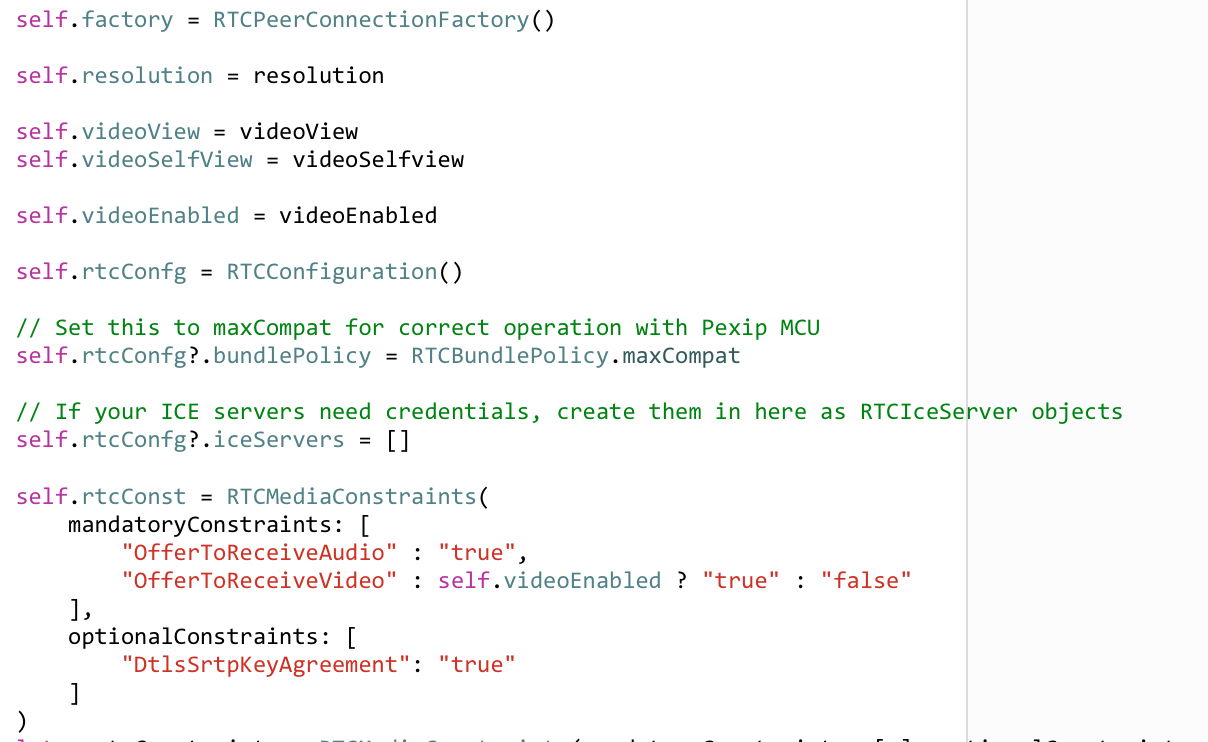
\includegraphics[width=.9\linewidth]{./images/peer_connection.png}
\end{center}


\subsubsection{Building media streams from tracks}
\label{sec:orgc7449c0}

\label{org08f246d}

Once we have our \texttt{RTCPeerConnectionFactory}, we can also use it to
create our media streams and assign our audio and video tracks to
them.  For iOS we'll be using \texttt{AVFoundation} sources and using the
\texttt{avFoundationVideoSource}, \texttt{videoTrack} and \texttt{audioTrack} methods of
the \texttt{RTCPeerConnectionFactory}.  For iOS, this could look like:

\begin{center}
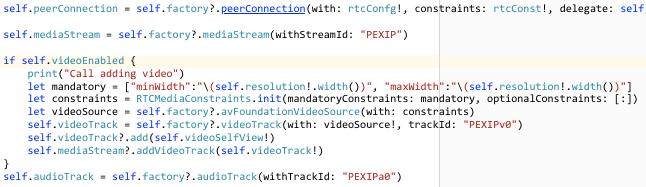
\includegraphics[width=.9\linewidth]{./images/add_tracks.png}
\end{center}

\subsubsection{Creating the offer with ICE candidates}
\label{sec:orgfa99b14}

Creating the offer using the \texttt{RTCPeerConnection} object will trigger a
bunch of calls that must be handled by your delegate in particular:

\begin{description}
\item[{RTCPeerConnection}] didChange newState RTCICEGatheringState
\end{description}

As this is what will return the final SDP back up to the application
so we can POST it to the MCU as our offer.  For iOS this could look like:

\begin{center}
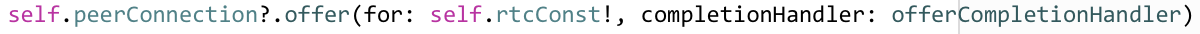
\includegraphics[width=.9\linewidth]{./images/peer_conn_offer.png}
\end{center}

\subsubsection{Mangling the SDP to set bandwidths and resolutions}
\label{sec:org5cbf104}

Before we POST the SDP to the MCU we must manipulate our SDP to set
the supported bandwidth and resolutions for the call e.g. make this a
wCIF call at 384kbps.  You could make this decision on behalf of your
user by looking at the connectivity of the device e.g. WiFi or
Cellular or through selection from user input e.g. "High Quality"
might convert to a 2Mbps call @720p.  Bear in mind that this is only
what is offered to the MCU, it might not actually end up being
negotiated and honored.  For more information, the reader is pointed
to \url{https://tools.ietf.org/html/rfc4566}.  We can mangle the SDP once we
reach the \texttt{RTCICEGatheringState.complete} i.e. all the ICE candidates
have been discovered and added to the description and we only really
need to set the \texttt{AS} and \texttt{TIAS} setting for the total session
bandwidth and the RTC constraints for capture device to set the out bound
resolutions (\texttt{minWidth}).  For iOS, this could look like:

\begin{center}
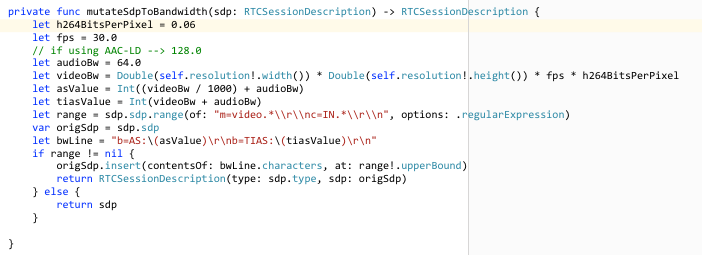
\includegraphics[width=.9\linewidth]{./images/sdp_mutation_functions.png}
\end{center}

\subsubsection{Sending the SDP offer}
\label{sec:org6291cff}

Once we have a complete offer with all candidates and we have
manipulated the SDP to what we want we can now POST this to the MCU.  
See \url{https://docs.pexip.com/api\_client/api\_rest.htm\#calls}

\subsubsection{Receiving the SDP answer}
\label{sec:org7e13dac}

Once the MCU has calculated an answer for for our offer, it will send
back its response and we can then manipulate this further e.g. to
limit the out bound bandwidth from our device and then pass this into
our \texttt{RTCPeerConnection} objects \texttt{remoteDescription}. For iOS, this
could look like:

\begin{center}
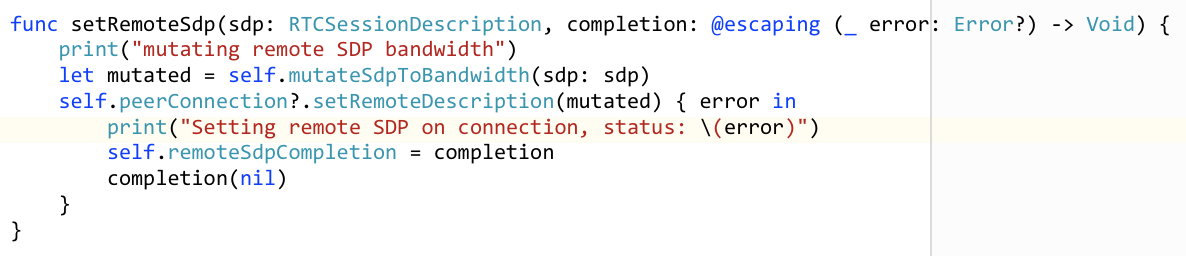
\includegraphics[width=.9\linewidth]{./images/remote_sdp.png}
\end{center}

\subsubsection{Connecting streams}
\label{sec:org7eab4e2}

Once our \texttt{RTCPeerConnection} objects \texttt{remoteDescription} has been set
and accepted you can now connect up the incoming streams to your views
to display the video and play the sound when the delegate function fires:

\begin{description}
\item[{RTCPeerConnection}] didAdd stream RTCMediaStream
\end{description}

In this event, you can pick out the audio and video streams and attach
them to your \texttt{RTCEAGLView} renderers i.e. the views you have setup to
show video in your app.  For iOS, this could look like:

\begin{center}
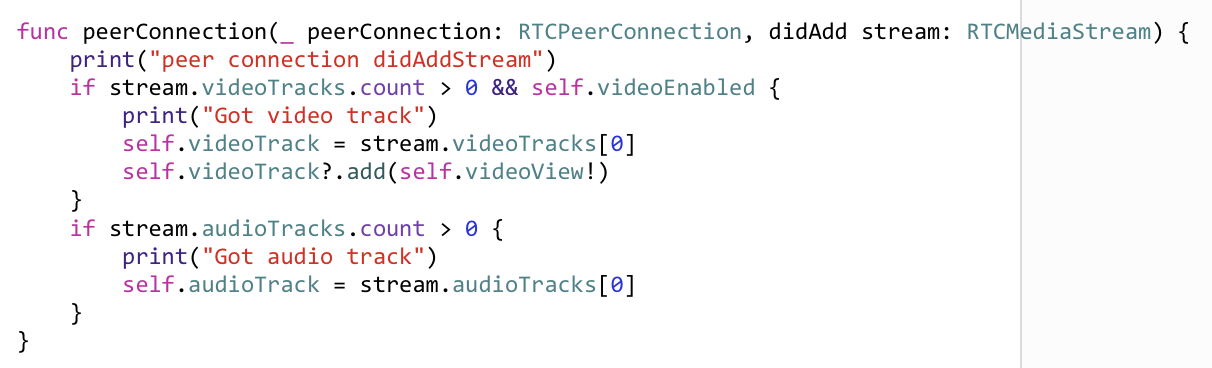
\includegraphics[width=.9\linewidth]{./images/add_stream.png}
\end{center}

\subsubsection{Starting media flow}
\label{sec:orga154fee}

Once the offer/answer dance has completed and you have wired up your
streams, you can know trigger the MCU into sending media by sending an
\texttt{ack} message: See \url{https://docs.pexip.com/api\_client/api\_rest.htm\#ack}.
Once this completes, you should start to see and hear media in your
application.

\subsubsection{Switching streams}
\label{sec:org19ec535}

You can switch tracks in the media stream to allow you to do things
like swapping between front and rear cameras.  You can do this using
\texttt{useBackCamera} on the \texttt{RTCAVFoundationVideoSource} e.g.:

\begin{center}
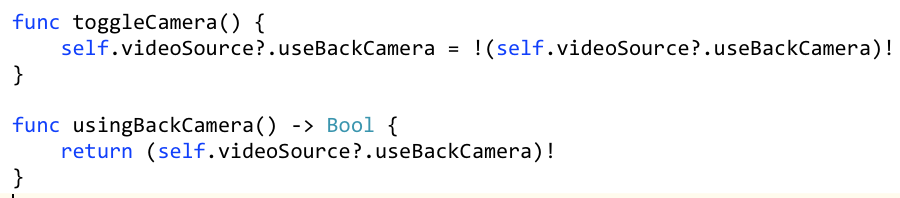
\includegraphics[width=.9\linewidth]{./images/toggle_camera.png}
\end{center}

\subsubsection{Crossing the streams}
\label{sec:orgaf146f8}

Never cross the streams, it would be bad.

\subsubsection{Disconnecting media flow}
\label{sec:orgfc2560e}

Once you have finished you can disconnect the media and drop back down
to an API participant.  See
\url{https://docs.pexip.com/api\_client/api\_rest.htm\#call\_disconnect}

\section{Platform Specific Considerations}
\label{sec:orgb3cfb24}
\subsection{iOS}
\label{sec:org98ea06c}
\subsubsection{WebRTC binaries}
\label{sec:org06d8d11}

At the time of writing, there is no native support for WebRTC in the
safari view controller so the only way to work with WebRTC is via a
binary install of the WebRTC library and rendering the results
using RTCEAGLViews in your UI.  You will need to build the WebRTC
library yourself (see Section \ref{org7558b4b} ) and then include the
header files in your project.  If you are using Swift, make sure that
a bridging header is in place to expose the bindings.  All examples
for this document will use Swift but the concepts transfer directly
for Objective-C based applications.

The library can be compiled with the full instruction set for use on
all ARM platforms and also with 386 and X86\_64 instructions for use in
the simulator.  You can control which platforms to target and hence
control the size of the included library.  When submitting to the App
Store, you \textbf{must} remove these non-ARM architectures from the
library or your app will be rejected.

\subsubsection{Bitcode}
\label{sec:orgb0f2682}

At the time of writing, there is also no support for Bitcode in the
library so you will need to disable this for your project.

\subsubsection{Hardware Acceleration}
\label{sec:orgc9474ae}

Hardware acceleration is enabled by default for the latest builds of
WebRTC and this should dramatically reduce the CPU load used when
decoding H264 streams but be aware that decoding video and audio is
still a very intensive workload and consideration should be taken when
deciding bandwidths and resolutions to negotiate with the MCU i.e. a
2Mbps stream at 720p HD resolution will require a modern ARM processor
and a lot of CPU power and older phones will struggle to decode this
in a timely manner.

On iOS devices with an A4 up to A6 processor, there is support for
H.264/AVC/MPEG-4 Part 10 (until profile 100 and up to level 5.1),
MPEG-4 Part 2, and H.263.  The A7 added support for H.264’s
profile 110.

\subsection{Android}
\label{sec:orgc7c126a}

For Android, there are actually two ways you can interact with WebRTC;
a web view with built in support for WebRTC that can be accessed via
JavaScript bindings; or using the same method as iOS with a WebRTC
library and a pure Java implementation.  See Sections
\ref{orgddd20c4} and \ref{orga2d90cc} for more
information.

\section{Building WebRTC}
\label{sec:org3a78d92}

\label{org7558b4b}

\subsection{Building WebRTC for iOS}
\label{sec:orga9c6f53}
\subsubsection{Custom patches for Pexip}
\label{sec:org69299e0}

At the time of writing, there is a custom patch to workaround support
for rotation of video streams that must be applied in order for the
video stream to be rotated to the correct orientation.  See Section
\ref{org89c5bf9} for links to the patches.

The reader is advised to use a "branch head" when building rather than
master as this is slightly more stable and reliable when building.  At
the time of writing, branch head 56 was used.

\begin{verbatim}
git checkout branch-heads/56
glclient sync
\end{verbatim}

We recommend building the framework as this greatly simplifies
addition to your project although if you want more fine grained
control, you can build the static library and only include what you
need.

\subsubsection{Building}
\label{sec:org6db1acd}

Building WebRTC for iOS must be performed on a Mac - these examples
were performed on a Macbook Pro running macOS 10.12.1.  The canonical
build instructions are \url{https://webrtc.org/native-code/ios/} but the
following process is a good summary.

\begin{enumerate}
\item Prerequisites
\label{sec:org6aeca14}
\begin{enumerate}
\item depot tools
\label{sec:orgfcb5068}

Clone the depot tools

\begin{verbatim}
git clone https://chromium.googlesource.com/chromium/tools/depot_tools.git
\end{verbatim}

Make sure they are in your path:

\begin{verbatim}
export PATH=`pwd`/depot_tools:$PATH
\end{verbatim}

\item WebRTC code
\label{sec:org7cf5cac}

Create a working directory, enter it and fetch the code:

\begin{verbatim}
mkdir ~/webrtc
cd ~/webrtc
fetch —nohooks webrtc_ios
\end{verbatim}

Now sync and pull down the code.  This will take a long time and
should not be interrupted as multiple gigabytes of data will be
downloaded.

\begin{verbatim}
gclient sync
\end{verbatim}
\end{enumerate}

\item Building
\label{sec:org4613ee4}
\label{orgb90e33c} Once you have the source (and have applied any
necessary patches) you can either build a static binary or a
framework.  Building a framework is the simpler option but the static
binary gives you more control.


\item Building the framework
\label{sec:org1750310}

\begin{verbatim}
cd ~/webrtc/src
\end{verbatim}

Build the framework:

\begin{verbatim}
./webrtc/build/ios/build_ios_libs.sh
\end{verbatim}

The result will be a directory called \texttt{out\_ios\_libs} containing the
framework called \texttt{WebRTC.framework}.  You can now embed this directly
into you project.

\item Building the static Binary
\label{sec:org7438bc4}

\begin{verbatim}
cd ~/webrtc/src
\end{verbatim}

Build the static binary:

\begin{verbatim}
./webrtc/build/ios/build_ios_libs.sh -b static_only -o out
\end{verbatim}

The result will be a library and a set of headers in the \texttt{out}
directory.

The \texttt{out} directory will contain a single \texttt{librtc\_sdk\_objc.a} with all
architectures combined and sub directories containing the individual
architectures.  The header files will be located in
\texttt{./webrtc/sdk/objc/Framework/Headers/WebRTC/}

If the build script fails you can run the compilation manually:

\begin{verbatim}
gn gen out/arm64 --args='target_os="ios" target_cpu="arm64" \
is_component_build=false is_debug=false’
gn gen out/arm --args='target_os="ios" target_cpu="arm" \ 
is_component_build=false is_debug=false’

ninja -C out/arm64 rtc_sdk_framework_objc
ninja -C out/arm rtc_sdk_framework_objc
\end{verbatim}


\begin{enumerate}
\item Adding WebRTC and headers to your Swift project
\label{sec:org9e17891}

\begin{enumerate}
\item Create a new group in your project hierarchy called WebRTC and
create a new header file called \texttt{<bundle id>-Bridging-Header.h}
\item Copy in the binary lib and headers created in the build process above.
\item Add the import lines to the bridging header
\begin{enumerate}
\item You can run the following command from the headers directory from Section \ref{orgb90e33c} to
get a listing ready to paste in:
\begin{verbatim}
ls *h | awk '{print "#import \"" $NF "\""}'
\end{verbatim}
You won't need all of these headers and the macOS ones can be
removed.
\end{enumerate}
\item Make sure \texttt{Build Settings -> Objective-C Bridging Header} has a
path set to the new bridging header you created
\item Include all the other frameworks and libraries required for proper
operation including your freshly built \texttt{librtc\_sdk\_objc} library,
in the following order:
\begin{itemize}
\item libresolv.tbd
\item AVFoundation.framework
\item CoreMedia.framework
\item GLKit.framework
\item OpenGLES.framework
\item CoreVideo.framework
\item CoreAudio.framework
\item QuartzCore.framework
\item AudioToolbox.framework
\item libc++.tbd
\item libstdc++.tbd
\item VideoToolbox.framework
\item librtc\_sdk\_objc.a
\end{itemize}
\end{enumerate}
\end{enumerate}
\end{enumerate}
\subsubsection{Other settings}
\label{sec:org8017736}

\begin{itemize}
\item Make sure the \texttt{Build Settings -> Other linker flags} is set to
\texttt{-ObjC} or you’ll get weird crashes about unknown signatures.
\item turn off bit-code support in \texttt{Build Settings}
\end{itemize}

\subsection{Building WebRTC for Android}
\label{sec:org953b2bc}

\label{orgddd20c4}

First, please take into account the design considerations mentioned in
Section \ref{orga2d90cc} as this will determine if you
even need to compile WebRTC for Android.

The canonical build instructions are here
\url{https://webrtc.org/native-code/android/} but at the time of writing are
still using the old \texttt{gyp} build system but the main repository has
moved over to the new \texttt{gn} build system.


\section{Example Code}
\label{sec:org1d029f8}
\label{org89c5bf9}

The example code is intended as a rudimentary guide to show you the
basic concepts for working with the API and it \textbf{should not be used as
a basis for your application} as, for example, it does no validation
of user input, no error checking for responses from the API, no proper
layout of the video elements, no care for proper background operation
and no translation of any user interface elements into other
languages.  The examples also do not follow any of the HIGs laid out
by Apple
(\url{https://developer.apple.com/ios/human-interface-guidelines/overview/design-principles/})
or Google (\url{https://developer.android.com/design/index.html})

The example code can be found in \url{https://github.com/pexip/pexkit-sdk}.

\subsection{License}
\label{sec:orgd269c8e}

All examples and code are released under the MIT license:

\begin{verbatim}
The MIT License (MIT)

Copyright (c) 2016 Pexip

Permission is hereby granted, free of charge, to any person obtaining
a copy of this software and associated documentation files (the
"Software"), to deal in the Software without restriction, including
without limitation the rights to use, copy, modify, merge, publish,
distribute, sub license, and/or sell copies of the Software, and to
permit persons to whom the Software is furnished to do so, subject to
the following conditions:

The above copyright notice and this permission notice shall be
included in all copies or substantial portions of the Software.

THE SOFTWARE IS PROVIDED "AS IS", WITHOUT WARRANTY OF ANY KIND,
EXPRESS OR IMPLIED, INCLUDING BUT NOT LIMITED TO THE WARRANTIES OF
MERCHANTABILITY, FITNESS FOR A PARTICULAR PURPOSE AND
NONINFRINGEMENT. IN NO EVENT SHALL THE AUTHORS OR COPYRIGHT HOLDERS BE
LIABLE FOR ANY CLAIM, DAMAGES OR OTHER LIABILITY, WHETHER IN AN ACTION
OF CONTRACT, TORT OR OTHERWISE, ARISING FROM, OUT OF OR IN CONNECTION
WITH THE SOFTWARE OR THE USE OR OTHER DEALINGS IN THE SOFTWARE.
\end{verbatim}

\subsection{iOS}
\label{sec:org0a534bf}
\subsubsection{Design Considerations}
\label{sec:org2b367de}
\label{orge4d2f65}
It's a good idea to encapsulate the Conference functionality
(e.g. token handling, event handling, chat, presentation and call
handling) into a single class and the Call functionality (dealing with
WebRTC) in another class.  You can also setup structures for important
pieces of information e.g. resolutions, service errors etc

\subsubsection{DNS SRV}
\label{sec:org2910bd6}
\label{org5032cb9}
We have provided an example DNS SRV code snippet that you may include
in your projects if you prefer not to implement your own.

\subsubsection{SSE}
\label{sec:org6446cfc}
A good example of an SSE implementation is
\url{https://github.com/inaka/EventSource}.  We have successfully used this
to connect to the Pexip SSE stream.

\subsubsection{Audio Routing}
\label{sec:org1eb172f}
By default, audio will be routed to the earpiece on the phone.  You
can override this using the \texttt{AVAudioSession} as below (\texttt{.Speaker} is
just an Enum for clarity)

\begin{center}
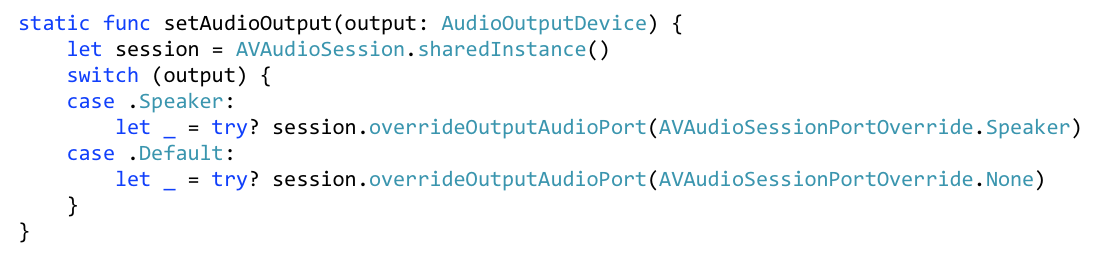
\includegraphics[width=.9\linewidth]{./images/audio_routing_swift.png}
\end{center}

You should modify this once the audio track has been established.

\subsubsection{Selfview}
\label{sec:org2a87206}
If you wish to display a self view (i.e. the local video track), you
can hook up another \texttt{RTCEAGLVideoView} to the video track as follows:

\begin{verbatim}
self.videoTrack?.add(self.videoSelfView!)
\end{verbatim}

This should be added in the initialisation of the call where you
create media streams.

\subsection{Android}
\label{sec:org9dfbfce}

\subsubsection{Design Considerations}
\label{sec:orgb0704a5}

\label{orga2d90cc}

As WebRTC is implemented in the Chrome web view for the Android
platform, there are a couple of options open to you when working with
WebRTC.  Firstly, you can work with the native web view and call the
REST API as the iOS client or you can use a wrapper around our PexRTC
JavaScript bindings to alleviate some of the work required.

The following examples assume you are using Android Studio and an API
Level of 21 or above.

\begin{enumerate}
\item To bundle PexRTC.js or not
\label{sec:org319e19d}

In order to use PexRTC.js you can either bundle the JavaScript with the wrapper project or fetch the JavaScript from your running deployment.

The wrapper includes a function called \texttt{fetchPexRTCSource} that will
pull in the running version of PexRTC on the targeted deployment.
You should make sure that any functions you are calling are still
supported in the current version.

The supplied wrapper already includes a bundled version of PexRTC, you
may need to update this every time you publish your app.

\item Building the wrapper
\label{sec:orgff7cd5f}

Simply open the supplied project and build it.  This will produce an
AAR file (in \texttt{pexrtc-android-wrapper/app/build/outputs/aar})
\end{enumerate}

\subsubsection{PexRTC wrapper}
\label{sec:org97e9792}

Import the wrapper library into your project using "File --> New -->
New Module" and select "import JAR/AAR package" from the selection.

Then navigate to the AAR wrapper file and import it.  Once complete,
you will now have this available in your resources side bar.

Open you project structure ("File --> Project Structure") then select
your existing "app" module and then select the dependencies tab and
add (+) a module dependency and select the AAR submodule you just
imported.

From your app, you should now be able to import
\texttt{com.pexip.android.wrapper.PexView} 

You can now add in your PexView (either or programmatically or via
adding it to your layout.xml file).

\begin{enumerate}
\item fragments vs normal view destruction
\label{sec:org4e0427c}

For configuration changes e.g. rotation, there are two methods of
dealing with the view destruction: use fragments or disable view
destruction (non-fragment way).

The following example uses the non-fragment method so you will need to
add the following line to your android manifest inside the activity:

\begin{verbatim}
android:configChanges="orientation|screenSize"
\end{verbatim}

e.g.

\begin{verbatim}
<activity android:name=".MainActivity"
     android:configChanges="orientation|screenSize" >
     <intent-filter>
     <action android:name="android.intent.action.MAIN" />

     <category android:name="android.intent.category.LAUNCHER" />
     </intent-filter>
 </activity>
\end{verbatim}

\item pro grammatic addition of PexView
\label{sec:orgcbbd3a9}

In your \texttt{onCreate} method of your main activity:

\begin{verbatim}
final PexView pexView = new PexView(this);
\end{verbatim}

Once you've have this, you can then grab the ID of your layout
(e.g. \texttt{myLayoutId}) from your layout XML file and then add the PexView
to it.

\begin{verbatim}
RelativeLayout layout = (RelativeLayout) findViewById(R.id.myLayoutId);
layout.addView(pexView);
\end{verbatim}

If you wish to show a self view:

\begin{verbatim}
WebView selfView = new WebView(this);
layout.addView(selfView);
pexView.setSelfView(selfView);
\end{verbatim}

\item addition via layout.xml
\label{sec:orgb2e9345}

Using the design view, add a custom view (search for PexView) and add
it where you see fit and then link them to your main activity e.g.

\begin{verbatim}
PexView pexView = (PexView) findViewById(R.id.pexViewId);
WebView selfView = (WebView) findViewById(R.id.selfViewID);
pexView.setSelfView(selfView);
\end{verbatim}

\item setting up callbacks for events
\label{sec:org1876b39}

Once you have your views setup, you can now register the callbacks for
the events from PexRTC e.g.

\begin{verbatim}
pexView.setEvent("onSetup", pexView.new PexEvent() {
	@Override
	public void onEvent(String[] strings) {
	    pexView.setSelfViewVideo(strings[0]);
	    pexView.evaluateFunction("connect");
	}
    });

pexView.setEvent("onConnect", pexView.new PexEvent() {
	@Override
	public void onEvent(String[] strings) {
	    if (strings.length > 0 && strings[0] != null)
		pexView.setVideo(strings[0]);
	}
    });

pexView.addPageLoadedCallback(pexView.new PexCallback() {
	@Override
	public void callback(String args) {
	    // make a call
	    pexView.evaluateFunction("makeCall", "pexipdemo.com", "meet.vmr", "My Display Name", "576");
	}
    });

// Load the page which will then trigger the callbacks
pexView.load();
\end{verbatim}

\item adding permissions to the android manifest
\label{sec:orgd2d2187}

You'll need the following permissions in your manifest file:

\begin{verbatim}
<uses-permission android:name="android.permission.INTERNET"/>
<uses-permission android:name="android.permission.CAMERA"/>
<uses-permission android:name="android.permission.MODIFY_AUDIO_SETTINGS"/>
<uses-permission android:name="android.permission.RECORD_AUDIO"/>
\end{verbatim}
\end{enumerate}

\subsubsection{Native}
\label{sec:org3089b9e}

Follow iOS instructions if you wish to go the native route.

\subsection{Cordova}
\label{sec:org3609769}

We have created a fork of the official Cordova plugin to work with the
latest WebRTC.  Access to these plugins will be made available at a
later date.
\end{document}
